\chapter{Medical and Technological Background}
\label{cha:background}

This chapter contains all the medical and technical information that can help in the further course of the work. We will cover key concepts related to heart rate, the 6MWT, body mass index, heart rate measurement with the Apple Watch and a comparison of various technical devices.

\section{Heart Rate}
Heart rate (HR) refers to the number of heartbeats per minute. When the body is at rest, this rate is called the resting heart rate. The resting heart rate is an important measure for assessing heart function and varies between individuals. It is a key indicator of cardiovascular health and physical fitness, with a normal resting heart rate ranging from 60 to 100 beats per minute ~\cite{heart}.

Various factors can affect heart rate, including age, sex, fitness level, medications, and underlying health conditions.

Even resting heart rate can differ among individuals. Women often have a slightly higher heart rate than men. Research by ~\textcite{HeartRate_study} shows that women's resting heart rates are typically 8-10 beats per minute higher than men's. For adult men, the average resting heart rate ranges from 70 to 72 beats per minute, while for adult women, it generally ranges from 78 to 82 beats per minute.

Women generally have smaller hearts than men, requiring a faster beat to circulate the same amount of blood. Additionally, studies like ~\textcite{Ryan1994GenderAA} suggest that women's heart pacemakers have a unique intrinsic rhythm, resulting in naturally faster heartbeats.

\section{6-Minute Walk Test}

The 6MWT is a practical and widely used measure of functional exercise capacity, as detailed by ~\textcite{6MWT}. 
It measures how far a patient can walk in six minutes, reflecting their ability to perform daily activities. This test provides an overall assessment of a patient’s respiratory, cardiovascular, neuromuscular, and cognitive functions. Unlike tests that measure maximal exercise capacity, the 6MWT evaluates a patient’s functional level during everyday activities ~\cite{6MWT}.

The American Thoracic Society's guidelines highlight the test's safety, ease of administration, and its better reflection of daily activities compared to other walk tests. 

The primary measurement is the 6-Minute Walk Distance (6MWD), but it also provides data on blood oxygen saturation and the patient's perception of exertion ~\cite{6MWT}.

The work by ~\textcite{6MW-ML} emphasizes the importance of accurately assessing dynamic balance ability in the elderly, critical for fall risk assessment and overall health monitoring. This research uses ML models to predict the age of elderly individuals based on their performance in the 6MWT, utilizing data from an Inertial Measurement Unit. The study collected data, extracted features related to movement and balance, and trained ML models like Random Forest (RF) and Gradient Boosting Machine (GBM) to predict the participants' ages. The combined features from both  Instrumented Timed Up and Go and 6MWT yielded the best performance, indicating a strong correlation between the Digital Biomarker Analysis and the chronological age. The study concludes that ML-enhanced 6MWT could be effective tools for Digital Biomarker Analysis assessment.

~\textcite{6MWtech} provide a systematic review of various studies using sensor technologies to monitor the 6MWT. The review covers studies from 2016 to 2021 and includes diseases like multiple sclerosis, pulmonary diseases, heart diseases, brain injuries, bone diseases, and kidney diseases. Most studies used motion and inertial sensors in devices, with some employing Diffusion Tensor Imaging and GPS technologies. The review highlights the importance of medical collaboration and the potential of sensor technologies for remote and continuous monitoring of 6MWT performance, enhancing patient care and disease management.

The paper by ~\textcite{ROMERO2022107020} outlines a methodology to predict 6MWT outcomes in Chronic Obstructive Pulmonary Disease patients using clinical and cardiopulmonary parameters without performing the test physically. The study collects data such as anthropometric data, spirometry parameters, and physiological data. It uses analytical techniques to extract heart rate variability indices from Electrocardiogram (ECG) data, incorporating these into a predictive model. The model employs lasso regularization for feature selection and ordinary least squares regression for final formation. Individual models estimate 6MWT outcomes like total distance walked, maximum heart rate achieved, and heart rate recovery, and a Bayesian network couples these models for simultaneous estimation. The models show moderate to strong correlations between predicted and actual measures, suggesting potential for remote patient monitoring and personalized care in Chronic Obstructive Pulmonary Disease patients where physical performance tests are not feasible.

\section{Body Mass Index}

The body mass index (BMI) is a widely used and straightforward index that calculates the ratio of weight to height to categorize individuals into different weight statuses. This method offers a quick way to assess potential health risks associated with body fat.

The World Health Organization (WHO) provides a standardized table and formula for BMI categorization, which has been instrumental in this research ~\cite{whoHealthyLifestyle}. The table below summarizes the WHO BMI categories:

\begin{table}[ht]
    \centering
\begin{tabular}{|l|r|}
\hline
\textbf{BMI} &  \textbf{nutritional status}  \\ \hline
< 18.5            &   underweight\\ \hline
18.4 - 24.9       &   normal weight \\ \hline
25.0 - 29.9       &   pre-obesity \\ \hline
30.0 – 34.9       &   obesity class I \\ \hline
35.0 – 39.9       &   obesity class II \\ \hline
> 39.9            &   obesity class III \\ \hline
\end{tabular}
\caption{WHO BMI categorization}
\label{table:BMI}
\end{table}

According to WHO guidelines, BMI categories help in identifying individuals at risk for health issues such as cardiovascular diseases, diabetes, and other conditions related to overweight and obesity ~\cite{whoHealthyLifestyle}. In this work, the guidelines of table ~\ref{table:BMI} are used to analyze the health risk of the participants and to add an additional health factor that can be quickly evaluated.

The formula for calculating BMI is the following:

\begin{equation}
    BMI = \frac{\text{weight (kg)}}{\text{height (m)}^2}
\end{equation}

This formula divides a person's weight in kilograms by the square of their height in meters, resulting in a value that can be used to determine their BMI category. By applying this formula, we can categorize individuals and assess their potential health risks based on the standardized BMI ranges provided by the WHO.

\section{Heart Rate Measurement with Apple Watch}

The Apple Watch uses advanced technology to measure heart rate. This section explains how the Apple Watch measures heart rate and the functionalities of these measurements ~\cite{AppleSupport120277}.

The main technology used in the Apple Watch for heart rate measurement is photoplethysmography. This technique works on the principle that blood reflects red light and absorbs green light. In detail it uses green LED lights and light-sensitive photodiodes to detect blood flow in the wrist. The green LEDs flash hundreds of times per second, allowing the Apple Watch to measure heart rate by observing changes in light absorption caused by blood flow. The optical heart sensor can measure heart rates between 30 to 210 beats per minute, adjusting the LED brightness and sampling rate for accuracy, even with low signal levels.

\FloatBarrier
\begin{figure}[h!]
\centering
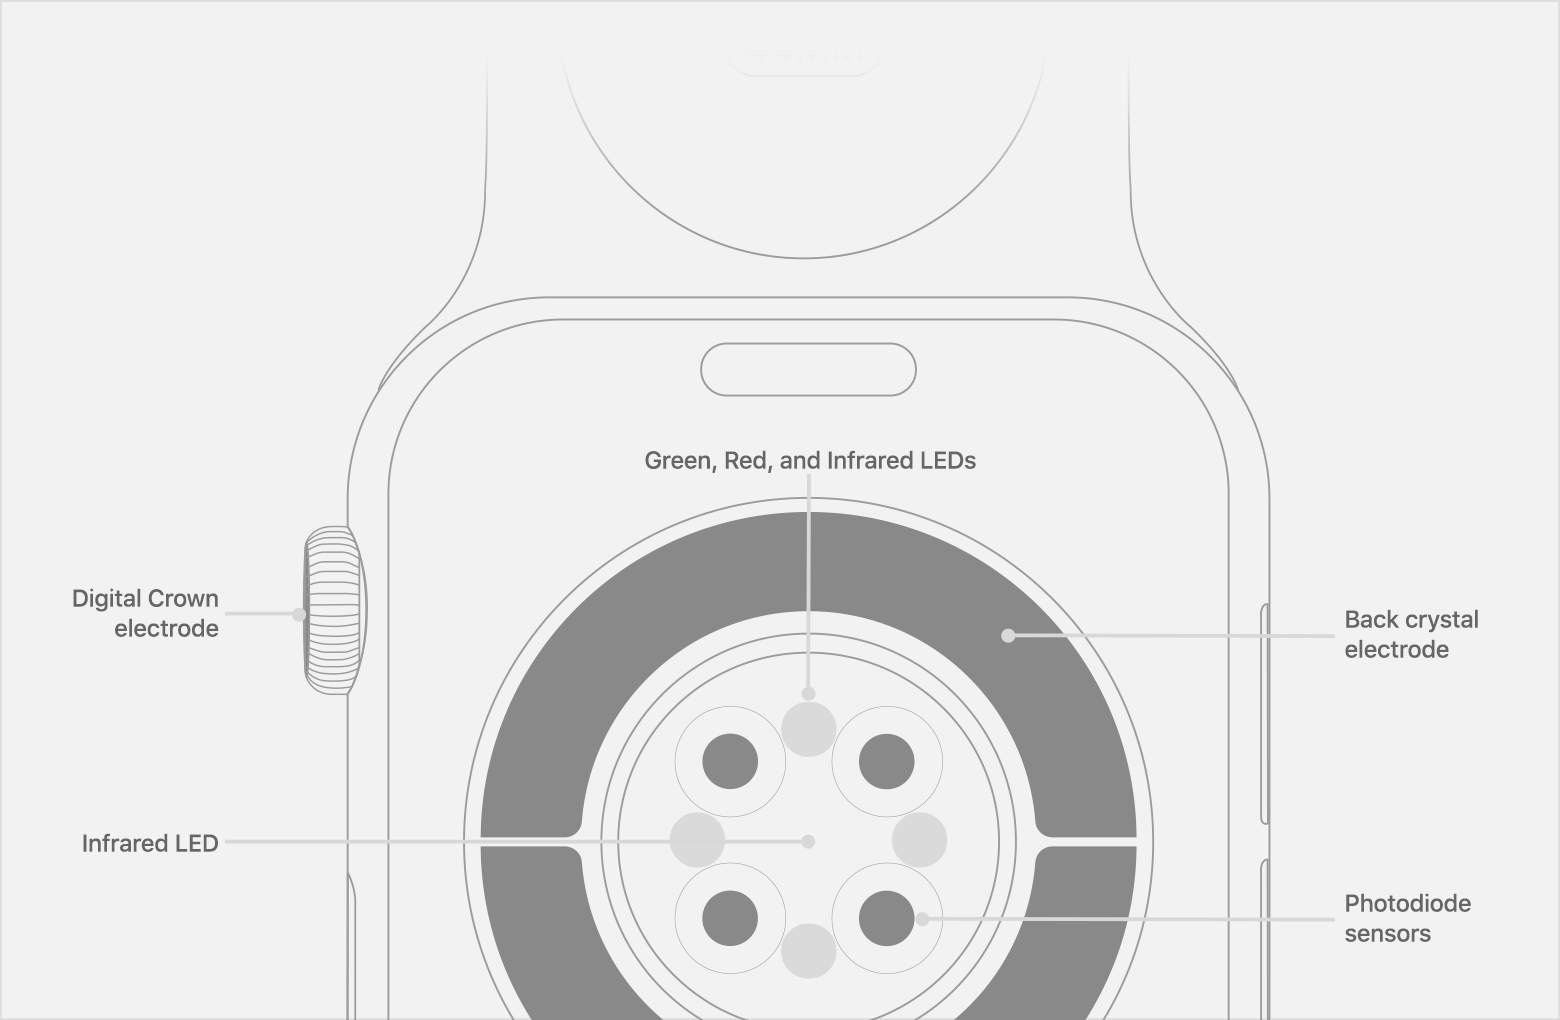
\includegraphics[width=0.85\textwidth]{Master Thesis/Plots/apple-watch-series6-measure-sensors.png}
\caption{Diagram of the Apple Watch sensors}
\label{fig:applewatch}
\end{figure}
\FloatBarrier

Figure ~\ref{fig:applewatch} shows the back of an Apple Watch, highlighting its sensors and components. It includes the 'Digital Crown Electrode' on the side and the 'Back Crystal Electrode' underneath for taking ECG readings. The Infrared LED, used for background heart rate measurement and notifications, is located around the sensor area. The central optical heart sensor, with green, red, and infrared LEDs, is essential for detecting blood flow and measuring heart rate. Photodiode sensors nearby detect reflected light from the skin to calculate heart rate. This setup enables the Apple Watch's comprehensive health monitoring features.

Besides using green LED lights, the optical heart sensor can also use infrared light for heart rate measurement. This mode is generally used for background heart rate monitoring and notifications. During active sessions such as workouts and Breathe sessions, the green LEDs are used to calculate metrics like walking average and heart rate variability ~\cite{AppleSupport120277}.

Starting with the Apple Watch Series 4 and including all models of the Apple Watch Ultra, the device features built-in electrodes in the 'Digital Crown' and the back of the watch. These electrodes measure electrical signals across the heart. When used with the Heart Rate app or the ECG app, placing a finger on the Digital Crown creates a closed circuit between the heart and both arms, capturing electrical impulses across the chest.

To use the electrical heart sensor for heart rate measurement, open the 'Heart Rate' app and place a finger on the 'Digital Crown'. This method provides a faster and more accurate reading, capturing data every second instead of every five seconds. Recorded data in the Health app will show 'ECG' in the 'Heart Rate' context ~\cite{AppleSupport120277}.

\section{Comparison to other Technical Devices}

The table below shows the performance of various fitness trackers in terms of distance and step count accuracy, as well as their battery life ~\cite{nytimesBestFitness}:

\FloatBarrier
\begin{table}[h!]
\centering
\begin{tabular}{|>{\raggedright}p{4cm}|>{\raggedright}p{2.5cm}|>{\raggedright}p{2cm}|>{\raggedright\arraybackslash}p{2cm}|}
\hline
\textbf{Product} & \textbf{Distance accuracy (miles)$^1$} & \textbf{Step count accuracy (\%)$^2$} & \textbf{Remaining battery life (48h)} \\
\hline
Amazfit Band 7 & $\downarrow$ 0.09 & $\uparrow$ 2 & 90\% \\
\hline
Apple Watch SE & $\downarrow$ 0.04 & $\uparrow$ 0.50 & 9\% (after 18 hours of testing) \\
\hline
Fitbit Charge 5 & $\downarrow$ 0.01 & $\uparrow$ 2 & 70\% \\
\hline
iPhone 15 & n/a & n/a & 0\% (after 20 hours of testing)\\
\hline
iPhone 13 mini & n/a & n/a & 0\% (after 17 hours of testing)\\
\hline
\multicolumn{4}{l}{\footnotesize{$^1$ According to 1-mile treadmill test (but without iPhone 13 mini and 15).
$^2$ \% error}}
\end{tabular}
\caption{Fitness tracker performance}
\end{table}
\FloatBarrier

The Fitbit Charge 5 stands out for its high accuracy in both distance and step counts, and a decent remaining battery life. The Apple Watch SE also performs well in terms of tracking accuracy but has a significantly shorter battery life compared to the other devices.

The data for the iPhone 13 mini and iPhone 15, while included for comparison, are marked as 'n/a'. This is because the rest of the table uses general values for continuous fitness tracking, and specific data for these values is not available. Although it is technically possible to obtain this information from our existing data, doing so would result in inconsistent references across the table.

In this study, we focus exclusively on the Apple Watch Ultra, emphasizing the new generation's capabilities in health monitoring and prediction through the use of ML, what we will define more detailed later. The aim of this study is to evaluate the accuracy and reliability of the Apple Watch's measurements and to explore both its potential and limitations.